\documentclass[a4paper,11pt]{jarticle}
% \usepackage{}

\title{文書タイトル}
\author{著者}
\date{\today}

\begin{document}
    \maketitle

    \clearpage
    \tableofcontents

    \clearpage
    \section{第1章}
        ここは第1章です.
        \subsection{第1節}
            ここは第1節です.
            \subsubsection{第1小節}
                ここは第1小節です.
                \paragraph{パラグラフ}
                    ここはパラグラフです.
                    \subparagraph{サブパラグラフ}
                        \label{sec:subparagraph}
                        ここはサブパラグラフです.

    \cleardoublepage
    \section{第2章}
        \begin{table}[h]
            \centering
            \caption{tab caption}
            \begin{tabular}{lr} \hline
                head1 & head2 \\\hline
                col11 & col12 \\
                col21 & col22 \\\hline
            \end{tabular}
            \label{tab:table}
        \end{table}

        \begin{table}[h]
            \caption{tab caption2}
            \begin{tabular}{cc} \toprule
                head1 & head2 \\\midrule
                col11 & col12 \\
                col21 & col22 \\\bottomrule
            \end{tabular}
            \label{tab:table2}
        \end{table}

        \begin{figure}[h]
            \centering
            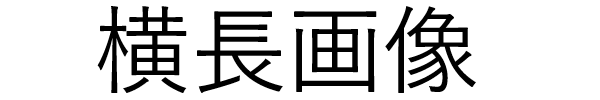
\includegraphics{zzz.png}
            \caption{fig caption}
            \label{fig:figure}
        \end{figure}

        \subsection*{コメントアウト}
            % コメントアウト
%コメントアウト
            途中で % コメントアウト
            これは \% コメントじゃないよ

\end{document}